\chapter{Design}\label{ch:design}
In this chapter we will provide an overview of how the defects in SiC can be used for \index{magnetometry}{magnetometry}, \index{thermometry}{thermometry} and \index{electrometry}{electrometry} in isolation. We will then develop a framework where by combining specific defects we may simultaneously measure multiple parameters. 

\section{$S=1$ Magnetometry}
We begin by considering a triplet state, that is a $S=1$ system. 

Under the influence of a magnetic field, the Hamiltonian can be expressed as: 
\begin{equation}
    H_{} = H_{\ce{D}} + H_{\ce{Z}}} 
    \label{eq:nv_hamil}
\end{equation}

Here the labels $\ce{D}$ and $\ce{Z}$ describe the electron spin-spin interactions and the Zeeman interaction with an external magnetic field. 

They have the following forms: 
\begin{eqnarray}
    H_{\ce{D}} &=& D S_z^2 + E(S_x^2 + S_y^2) \label{H_D} \\
    H_{\ce{Z}} &=& g \mu_B \sum_{j}^{x,y,z} B_j \cdot S_j \label{H_Z} \\
\end{eqnarray}

\subsubsection{Spin-Spin Interaction}

The $E$ and $D$ in equation \ref{H_D} represent the fine structure constants of the spin
system, describing the spin-spin interaction and $S_j$ the corresponding spin operators
in x,y and z-direction. 

$D$ is non-zero in system with axis of threefold (or other manifold) symmetry. 
The definiteness, orientation and magnitude of $D$ is dependent on the specific spin system being studied. 

$E$ occurs when there is a distortion of the point group symmetry, for example strain or an $\vec{E}$ field. 
Similarly, the value of $E$ is a characteristic of the nature of the distortion and 
the specifics of the spin system being studied. 

\subsubsection{Zeeman Interaction}

$B_j$ in equation \ref{H_Z} is the magnetic field along the $x$, $y$ and $z$ direction, $g$ is the $g$-factor of the vacancy and $\mu_B$ the Bohr-Magneton. 

% It seems often the scaled parameter $g\mu_B$ is considered, for the $\ce{NV^-}$ system this is around $28\;\ce{ GHz T^{-1}}$, but again, will be a characteristic of the system being studied. 

% \subsubsection{Reduced Hamiltonian}
By combining $H_{\ce{D}}$ and $H_{\ce{Z}}$ 
we find 
\begin{equation}
    H_{} = D S_z^2 + E(S_x^2 + S_y^2) + g \mu_B \sum_{j}^{x,y,z} B_j \cdot S_j 
    \label{eq:reduced_H_NV}
\end{equation}

the $S=1$ spin operators \eqref{eq:s1_spin_operators}, then aligning the magnetic field (with strength $B_0$) along the $z$-axis (the quantisation axis), the reduced Hamiltonian will have the form 
\begin{equation}
    H_{} = \begin{pmatrix}
        D + B_0 & 0 & E \\ 
        0 & 0 & 0 \\ 
        E & 0 & D-B_0
    \end{pmatrix},
    \label{eq:reduced_H_NV_matrix}
\end{equation}

with Eigenvalues 

\begin{equation}
    E_x = E_y = D \pm \sqrt{B_0^2  + E^2}, \; E_z = 0.
    \label{eq:reduced_H_NV_eigenvalues}
\end{equation}

The corresponding non-normalised Eigenvectors are then 

\begin{eqnarray}
    \ket{X} = \frac{1}{E} \left(B_0 + \sqrt{B_0^2 + E^2}\right) \ket{+1} + \ket{-1} \\ 
    \ket{Y} = \frac{1}{E} \left(B_0 - \sqrt{B_0^2 + E^2}\right) \ket{+1} + \ket{-1} \\ 
    \ket{Z} = \ket{0},
\end{eqnarray}
with
\begin{equation}
    \ket{1} = \begin{pmatrix}
        1 & 0 & 0 
    \end{pmatrix}, \; 
    \ket{0} = \begin{pmatrix}
        0 & 1 & 0 
    \end{pmatrix}\;, 
    \ket{-1} = \begin{pmatrix}
        0 & 0 & 1 
    \end{pmatrix},
    \label{eq:base_states}
\end{equation}
the Eigenvectors for $H$ with $E=0$ \td{Need to finish write up. }.

In the case where $E \ll B_0$ the Eigenvectors are well described by the bases $\ket{0}$ and $\ket{\pm 1}$.

For an arbitrary external magnetic field, $H$ can be expressed using spherical co-ordinates: 
\begin{equation}
    H = \begin{pmatrix}
        D + B_0 \cdot \cos \theta & \frac{B_0}{\sqrt{2}} \cdot e^{-i\cdot \varphi} \cdot \sin\theta & E \\ 
        \frac{B_0}{\sqrt{2}} \cdot e^{i \cdot \varphi} \cdot \sin\theta & 0 & \frac{B_0}{\sqrt{2}} e^{-i\cdot \varphi} \cdot \sin\theta \\ 
        E & \frac{B_0}{\sqrt{2}} \cdot e^{i \cdot \varphi} \cdot \sin\theta & D - B_0 \cdot \cos \theta
    \end{pmatrix}
    \label{eq:nv_hamil_spherical_matrix}
\end{equation}


Here, we transformed the magnitude of the arbitrary magnetic field into spherical co-ordinates as 
\begin{eqnarray}
    B_x  &=& B_0 \cos\varphi \sin\theta \\ 
    B_y  &=& B_0 \sin\varphi \sin\theta \\ 
    B_z  &=& B_0 \cos\theta 
\end{eqnarray}
with $\theta$ the azimuthal and $\varphi$ the polar angle. Then using equations \ref{eq:reduced_H_NV} and \ref{eq:spin_operators} we compute \ref{eq:nv_hamil_spherical_matrix}.  

It immediately follows from the characteristic \td{need to finish writing this} equation that Eigenvalues $\lambda$ satisfy 
\begin{equation}
    0 = \lambda^3 - 2\cdot \lambda^2 \cdot D + \frac{D \cdot B_0^2}{2} + \lambda(D^2 - E^2 - B_0^2) - \frac{1}{2}B_0^2\underbrace{\left(D \cdot \cos(2\theta) - 2 \cdot E \cos(2\varphi) \cdot \sin(\theta)^2\right)}_{\Delta_{\varphi \theta}}
    \label{eq:nv_spherical_characteristic_equation}
\end{equation}
% \cite{balasubramanian2009}




% https://magnetometryrp.quantumtinkerer.tudelft.nl/3_NVspin/


\subsection{$\vec{B}$ Parallel to Defect Axis}
The simplest implementation of the magnetometer is when the applied magnetic field, $B_0$ is parallel to the defect axis. 

In this case, the entire magnitude of the field contributes to the Zeeman splitting of the energy level. This means in the CW-ODMR spectra the difference between the two frequencies $f_1 > f_2$ is directly proportional to $B_0$ and related as detailed in Section \ref{zeeman}.
$$f_1 = D + \gamma B_0,  \quad f_2 = D - \gamma B_0$$
It is then straightforward to calculate $B_0$ using 
$$B_0 = \frac{f_1 - f_2}{2 \gamma} $$
which is visualised for the DNV system in figure \ref{fig:spin1_magnetometry}. 
% \begin{wrapfigure}{r}{0.5\textwidth}%
%     \centering%
%     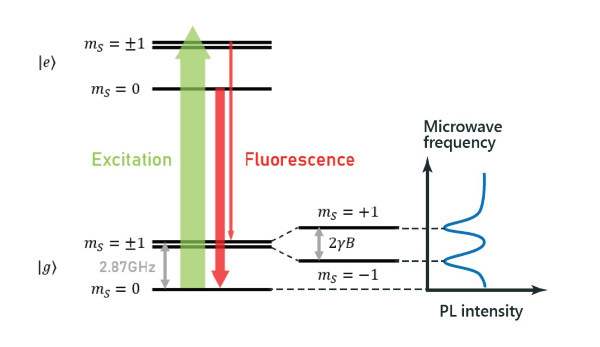
\includegraphics[width=0.5\textwidth]{figures/NVlevelwithESR.png}
%     % 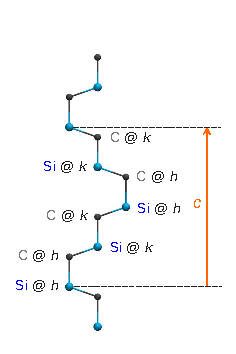
\includegraphics[width=0.38\textwidth]{figures/SiC-non-equiv-sites.pdf}%
%   \caption{Magnetometry with $\theta = 0$. Left shows the lifting of degeneracy of the spin system energy levels with the applied $\vec{B}$ field. Right shows the corresponding ODMR spectra and two EPR frequencies \cite{dnvweb}. \td{better caption}}%
% \label{fig:spin1_magnetometry}
% \end{wrapfigure}

\begin{figure}[h]
    \begin{center}
    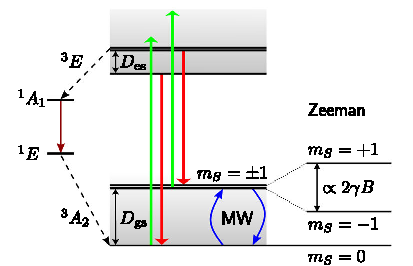
\includegraphics[width=0.7\textwidth]{figures/DNV-ODMR.pdf}
% \missingfigure{Two panel figure. Panel 1 - energy level splitting of S=1 system being prop to gyromagnetic ratio. Panel 2 - ODMR Spectra} 
    \end{center}
    \caption{ODMR Magnetometry with $\theta = 0$. Degeneracy of the spin system energy levels is lifted with the applied $\vec{B}$ field \cite{Strner2021}. }
\label{fig:spin1_magnetometry}
\end{figure}
%

\subsubsection{$\vec{B}$ at Angle $\theta$ to Defect Axis}
The Zeeman effect is proportional to $\cos\theta$, thus, when $\vec{B}$ is perpendicular to the defect axis the Zeeman effect reduces to zero, varying the azimuthal angle $\theta$ is effectively the same as scaling $B_0$ by $\cos \theta$. 

\begin{figure}[h]
    \begin{center}
 % /        \missingfigure{ODMR or Energy Eigenvalues plot for $\theta = 0, 30, 60, 90$ showing the effective reduction of applied parallel field.}
    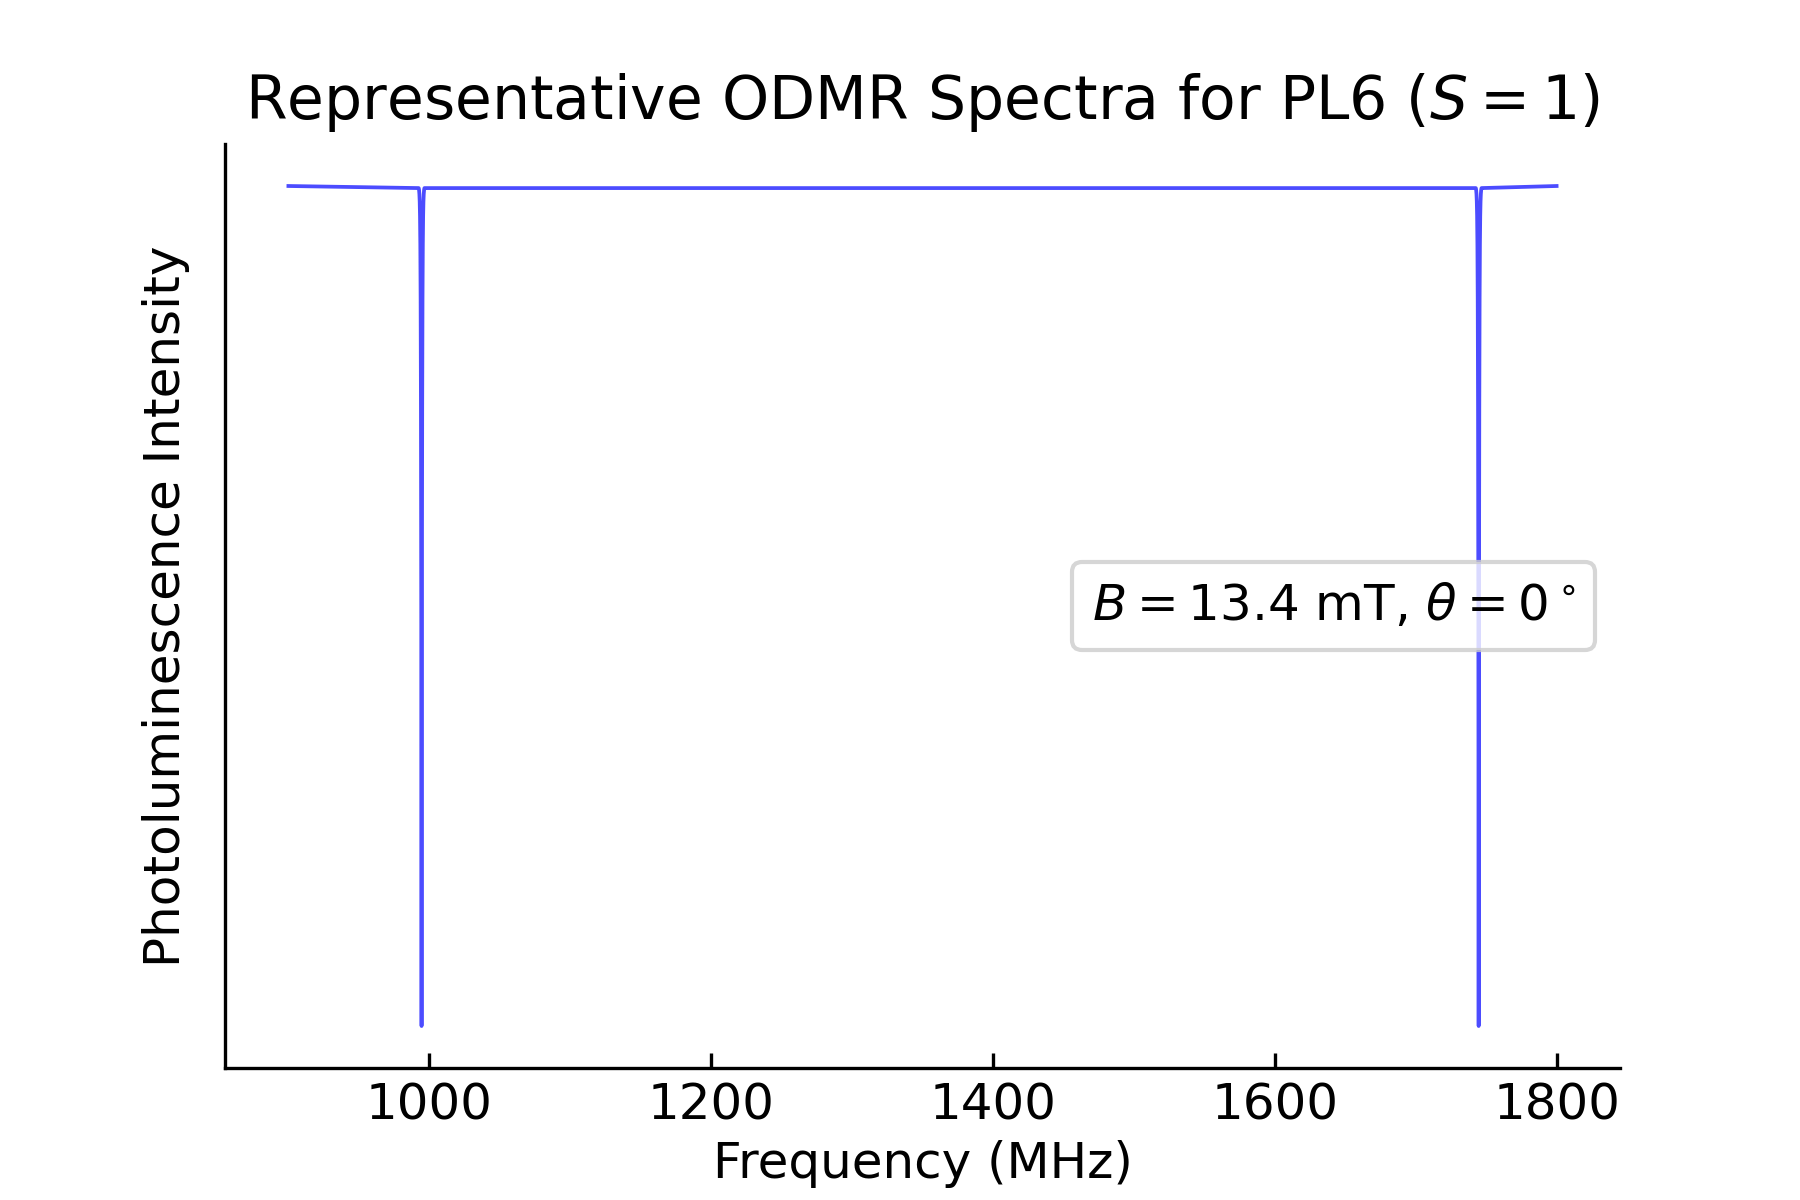
\includegraphics[width=\textwidth]{figures/PL6ODMRSpectra_theta_0_to_90.png}
    \end{center}
    \caption{ODMR/Energy level plot showing the reduction of the effective parallel $\vec{B}$ field with increasing $\theta$.} 
    \label{fig:}
\end{figure}


\subsection{$S=1$ Vector Magnetometry}
Vector magnetometry with a $S=1$ system can be achieved by comparing the relative intensities from defects known to be at specific angles. 

For example, in diamond the nitrogen vacancy is aligned with the tetragonal crystal structure and thus may take one of four orientations as illustrated in Figure \ref{fig:dnv_orientations}. 

\begin{figure}[h]
    \begin{center}
        % \missingfigure{Sketch of DNV and possible defect orientations.}
        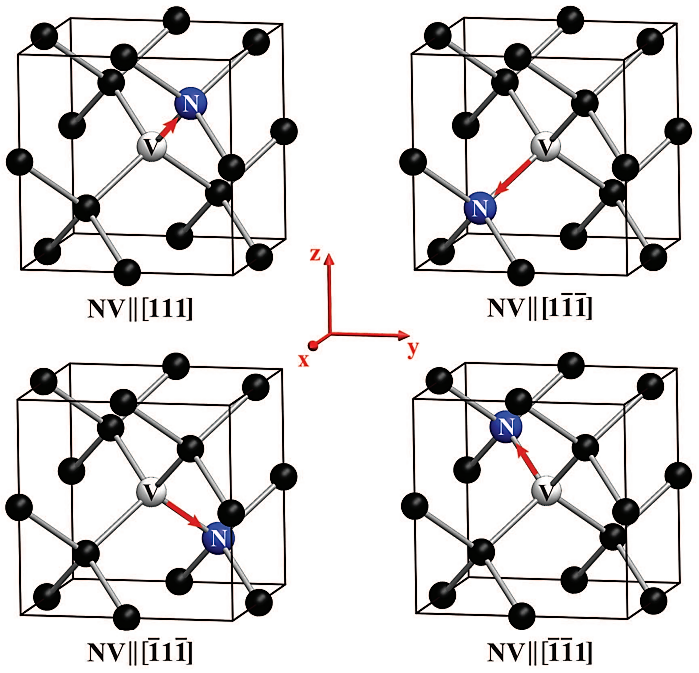
\includegraphics[width=0.45\textwidth]{figures/four_possible_NV_orientations.png}
    \end{center}
    \caption{Diagram showing the four possible orientations of NV centers in diamond \cite{pham}.}\label{fig:dnv_orientations}
\end{figure}


The 4 possible DNV orientations in the lattice are $111$, $1\overline{11}$, $\overline{1}1\overline{1}$ and $\overline{11}1$. 
Once the projections of the magnetic field along these axes have been measures, we reconstruct the magnetic field in the laboratory frame.

The ODMR sprectrum for a sample of diamond with approximately equal distribution of the four defect orientations. 

% # file:///home/conner/Downloads/e2015-60080-1.pdf
\td{Finish typing - link in comments}
The measured field components $m_i$ do not directly give the magnetic field $B_i$, but are affected by some noise in-
herent to the measurement which is accounted for using a maximum-likelihood method. 

% The direction of $\vec{B}$ relative to the crystal lattice can then be determined by solving 
% \begin{equation}
%     \underbrace{
%     \frac{1}{\sqrt{3}}
%     \begin{pmatrix}        
%         1 & 1 & 1 \\ 
%         -1 & -1 & 1 \\ 
%         -1 & 1 & -1 \\ 
%         1 & -1 & -1 
% \end{pmatrix}}_{N}
%     \mathbf{\hat{B}} = 
%     \underbrace{
%     \begin{pmatrix}
%         \cos\theta_1 \\
%         \cos\theta_2 \\
%         \cos\theta_3 \\
%         \cos\theta_4 \\
%     \end{pmatrix}
% }_{\mathbf{c}}
%     \label{eq:}
% \end{equation}
% For which a solution may be determined 
% \begin{equation}
%     \mathbf{\hat{B}} = \left(N^T N\right)^{-1} N^T \mathbf{c}.   
%     \label{eq:}
% \end{equation}
%
% With knowledge of .. \td{Need to finish writing about knowing the miller index family of crystal can convert miller vector to lab vector}. 
%

\cite{Balasubramanian2008}
\td{Need to also look at this method and type up}

\section{$S = 3/2$ Magnetometry}
% V2 
\cite{PhysRevApplied.4.014009}
\cite{PhysRevB.92.115201}
\cite{1505.06914}

If the ZFS interaction of the $S=3/2$ defect is sufficiently strong, the eigenvalues of the
spin Hamiltonian show a strong dependence on the orientation of the applied magnetic field. 

This induces a non-linear shift of resonance transitions in EPR frequencies, which is seen in the ODMR spectra. 
This allows information about the applied external magnetic field to be extracted from ESR spectra provided the ZFS is known. 

In zero magnetic field the $V_{\ce{Si}}$ V2 vacancy has an ODMR line maximum around 70 MHz with very weak dependence on temperature. That is, the ZFS parameter is known and resistant to the environmental influence of temperature. 

In a $S=3/2$ spin system the orientation related terms are, like for $S=1$ systems, in the eigenvalue equation. 
This results in the orientation dependent shift of EPR frequencies which are not explained by $g \mu_B B_0$ as they are for $S=1$. 

Therefore in order to reconstruct the energy eigenstates we must use the observed resonant energies. There are $2S +1 $ states for a system with spin $S$ from which $2S$ transition frequencies may be found. 


% Applying a magnetic field $B_0$ along the defect axis, $\theta = 0$, 

For the V2 $V_{\ce{Si}}$, $E \ll D$ and a uniaxial symmetry exists therefore the Hamiltonian for the system is given as in equation \ref{}\td{ref correct hamiltonian}. Here we use the 4-dimensional $S=3/2$ matrix representation 
\begin{equation}
    \label{eq:}
\end{equation}
    \td{Add spin 3/2 matrices} 

    For this defect, using the same polar co-ordinate conversion as in section \ref{}\td{find ref} we may write the Hamiltionian in matrix form \td{Add hamiltonian matrix} and find the eigenvalue equation 
\begin{equation}
    \begin{align}
    &\lambda^4 - \left(2D^2 + 6E^2  + \frac{5}{2}(g\mu_B B_0)^2 \right)\lambda^2 - 2 (g \mu_B B_0)^2 \left(D(3 \cos^2 \theta -1) + 3E \sin^2\theta \cos 2\varphi \right)\lambda \\ 
    &+\frac{9}{16}(g \mu_B B_0)^4 + D^4 - \frac{1}{2}D^2 (g \mu_B B_0)^2 - D^2 (g \mu_B B_0)^2 (3 \cos^2 \theta - 1) + 3E^2(3E^2 + 2D^2) \\ 
    &+ E(g\mu_BB_0)^2 (6D \sin^2\theta \cos 2\varphi + \frac{9}{2}E \cos2\theta) = 0 
    \end{align} 
    \label{eq:V2_eigenvalue_equation}
\end{equation}
 
Considering $B_0$ componentwise we may find \cite{Kirmse1995} for $B_0$ parallel to the defect axis 
\begin{equation}
\lambda = \frac{1}{2}g\mu_B B_0 \pm \sqrt{(D + g\mu_B B_0)^2 + 3E^2} 
   \text{ or, }
   \lambda = -\frac{1}{2} g\mu_B B_0 \pm \sqrt{(D-g\mu_B B_0)^2 + 3E^2}.
    % \label{eq:}
\end{equation}

For $B_0$ perpendicular to the defect axis we find:
\begin{equation}
    \begin{align}
        &\lambda = \frac{1}{2}g\mu_B B_0 \pm \sqrt{(g\mu_B B_0)^2 + D^2  + 3E^2 - (D - 3E)g\mu_B B_0}\text{ or, }\\
        \lambda &= -\frac{1}{2}g\mu_B B_0 \pm \sqrt{(g\mu_B B_0)^2 + D^2 + 3E^2 + (D-3E)g\mu_B B_0}.
    \end{align}
\end{equation}

We may write the general equation for the eigenvalues as 
\begin{equation}
    \sum_{n=0}^{2S+1} C_n \lambda^n = 0
    \label{eq:}
\end{equation}
we then substitute each eigenvalue $\lambda_i$ into this general expression to obtain $2S + 1$ equations. 

The goal is now to remove all $\lambda_i$ terms by considering instead the transition frequencies between eigenstates, which are observed in the ODMR spectra. The energy states are not in general sorted with respect to the energy values, so we use the convention that $\lambda_i > \lambda_{i-1}$. 

To reduce our number of equations to $2S-1$ we make the substitutions  
$$\lambda_i + \underbrace{\lambda_{i+1} - \lambda_{i}}_{f_{i+1, i}} = \lambda_{i+1},
\qquad\lambda_i - \underbrace{(\lambda_{i} - \lambda_{i-1})}_{f_{i, i-1}} = \lambda_{i-1}$$
for each $i = 2, \dots, 2S$ and calculate both 
$$\sum_{n=0}^{2S +1} \frac{C_n \left((\lambda_i + f_{i+1, i})^n - \lambda_i^n\right)}{C_{2S+1}} = 0\text{ and } \sum_{n=0}^{2S +1}\frac{C_n \left((\lambda_i - f_{i, i-1})^n - \lambda_i^n\right)}{C_{2S + 1}} = 0$$
to find two new simultaneous equations 
$$\sum_{n=0}^{2S} C_{i,n}' \lambda_i^n = 0 \text{ and } \sum_{n=0}^{2S} C''_{i,n}\lambda_i^n = 0.$$

We may combine these as 
$$\sum_{n=0}^{2S} \frac{C'_{i,n}\lambda_i^n}{C'_{i,2S}}-\frac{C''_{i,n} \lambda_i^n}{C''_{i, 2S}} = 0$$
to obtain an equation for the eigenvalue of the energy eigenstate $\ket{i}$ where $i = 2, \dots, 2S$: 

\begin{equation}
    \sum_{n=0}^{2S -1} C_{i,n}^{(2S-1)} \lambda_i^n = 0.
    \label{eq:refmenowpls}
\end{equation}

This process is repeated until only one linear equation exists for each eigenvalue, which may be expressed in terms of resonant energies. $f_{i, i-1}$ can then be substituted to find expressions for all other eigenvalues. 

For the V2 $V_{\ce{Si}}$, we obtain equations for $\lambda_2$ expressed in terms of $f_{2,1}, f_{3,2}$ and $\lambda_3$ expressed in terms of $f_{3,2}, f_{4,3}$. Finally, using $f_{3,2} = \lambda_3 - \lambda_2$ we find formulas for each eigenvalues in terms of the resonant frequencies: 

\begin{eqnarray}
    \lambda_1 = -\frac{3}{4}f_{2,1} - \frac{1}{2} f_{3,2} - \frac{1}{4} f_{4,3}\\ 
    \lambda_2 = \frac{1}{4}f_{2,1} - \frac{1}{2}f_{3,2} - \frac{1}{4} f_{4,3} \\ 
    \lambda_3 = \frac{1}{4}f_{2,1} + \frac{1}{2}f_{3,2} - \frac{1}{4} f_{4,3} \\ 
    \lambda_4 = \frac{1}{4}f_{2,1} + \frac{1}{2}f_{3,2} + \frac{1}{4} f_{4,3}.
\end{eqnarray}

We substitute one of these expressions into one of the equations of the form of equation \eqref{eq:refmenowpls} and we obtain 
\begin{equation}
    \begin{align}
        5(g\mu_B B_0)^2 &=\left(\frac{\sqrt{3}}{2}f_{4,3} + f_{3,2}  + \frac{\sqrt{3}}{2}f_{2,1}\right)^2 \\ 
        &+(1 - \sqrt{3}) (f_{4,3} + f_{2,1})f_{3,2} - f_{4,3}f_{2,1} - 4(D^2 + 3E^2).
    \end{align}
    \label{eq:V2_magnitude}
\end{equation}

A second quantity $\eta$, useful for angle resolution (next section) related to the polar and azimuthal angle is also defined

\begin{equation}
        \eta \equiv E(2\cos^2\varphi \sin^2 \theta + \cos^2\theta) + D\cos^2 \theta 
    \label{eq:eta}
\end{equation}

which in terms of the resonant frequencies is given by 
\begin{equation}
    \begin{align}
    &\eta = \\ 
    &\frac{4\left(8(D + 3E) + 5(f_{4,3}-f_{2,1})\right)(g\mu_B B_0)^2 + (f_{4,3} - f_{2,1})\left(16(D^2 + 3E^2) - (f_{4,3}-f_{2,1})^2 - 4f_{3,2}^2\right)}{96(g\mu_B B_0)^2}
\end{align}
    \label{eq:eta_resonant}

\end{equation}


Overall, this shows that if the ZFS is known and three EPR frequencies are observed, the applied magnetic field strength can be found using \eqref{eq:V2_magnitude}.


% \subsection{$\vec{B}$ Parallel to Defect Axis}

% The simplest possible cashen $\theta = 0$ there is no super-position of states and selection rules dictate that the only transitions available 

\subsection{$S=3/2$ Angle Resolved Magnetometry}
We may approximate $\eta$ defined in equation \eqref{eq:eta} for the V2 $V_{\ce{Si}}$, which exhibits uniaxial symmetry, i,e, $E\ll D$, to 
\begin{equation}
    \eta \sim D \cos^2 \theta. 
    \label{eq:}
\end{equation}

By exploiting this approximation, we may also determine the polar angle that the magnetic field vector makes with the defect axis, however at this stage we may not determine anything about the $x,y$ components of the vector. 

To do so we explicitly compute $\eta$ using equation \eqref{eq:eta_resonant} then we find the polar angle as 
\begin{equation}
    \theta = \cos^{-1}\sqrt{\frac{\eta}{D}}
    \label{eq:vector_theta}
\end{equation}


\subsection{$S = 3/2$ Vector Magnetometry}
Vector magnetometry is achieved in the case of the DNV as described in section \ref{dnv_vector} \td{link reference} and theoretically a similar approach is possible in SiC. There exists two distinct and differently oriented Silicon vacancies in 4H-SiC and three in 6H-SiC \cite{Janzn2009}. In practice however, in practice at least one of the defects in each polytope is difficult to observe at room temperature making this approach unsuitable for vector magnetometry. 

In a general $S = 3/2$ system, ambiguity is found when computing $\theta$ using equation \eqref{eq:vector_theta} as the EPR frequencies can not be mapped to specific transitions. 

The following approach exploits the fact that a crossing of resonant frequencies occurs at a given angle (see figure \ref{fig:resonant_crossing_V2}). The method should be considered for $g\mu_B B_0 \gg 2\sqrt{D^2 + 3E^2}$ explicitly as interactions such as level anti-crossing produce a complex spectra \cite{Degen2008} when $g\mu_B B_0 \approx 2\sqrt{D^2 + 3E^2}$ and the invariance of a particular EPR frequency when $g \mu_B B_0 \ll 2 \sqrt{D^2 + 3E^2}$ makes determination of the polar angle $\theta$ impossible. 

\begin{figure}[h]
    \begin{center}
        % \includegraphics[width=0.95\textwidth]{figures/}
        \missingfigure{Plot showing the crossing of EPR frequencies at high field and low field in Spin 3/2 system as theta varies}
    \end{center}
    \caption{}\label{fig:resonant_crossing_V2}
\end{figure}
\begin{group}
    \color{gray}
At a high B0 field (gμB B0  ZFS),
B0 can be obtained from the observed ESR spectra but
the polar angle cannot be determined due to the ambigu-
ity of differentiating two outer transitions. In contrast,
at low gμB B0 ( ZFS), as long as one can explicitly
identify at least three transitions including the allowed
lowest energy transition, the external magnetic field vec-
tor can be reconstructed. In the field strength compara-
ble to the ZFS, it is hard to find a useful scheme because
very complex patterns appear due to mixing of some of
the eigenstates. In the case of the NV centers in dia-
mond (ZFS/h=2.87 GHz), this missing range is around
∼ 100 mT . The VSi in SiC can fill out this gap since its
ZFS is quite small (ZFS/h ∼ 100 MHz) thus this mag-
netic field range can be considered as a high field range
in which the three necessary transitions are well observ-
able25,29, and at least the field strength can be experi-
mentally determined. When the VSi in SiC is used to
realize such schemes at sub-mT, if the lowest transition
energy is observable by ELDOR, one can determine both
B0 and θ without ambiguity. 
% Even if ELDOR is not avail-
% able, thanks to the additional transitions that appear at
% low fields, the field strength can be determined.
% The magic angle terms in the eigenvalue equation al-
% low for an alternative method to use S=3/2 systems as
% a DC vector magnetometer. If the S=3/2 spins fixed
% in a crystal can be rotated around the rotational axis,
% the unambiguous determination of the applied magnetic
% field vector is feasible by monitoring the linewidth of the
% observed ESR spectra while the symmetry axis of the
% crystal is oriented at θm relative to the rotational axis
% and the rotational axis is moving. This configuration
% also can be realized by producing an array of the crystals
% such that the symmetry axes of each crystal form a cone
% whose opening angle is twice the magic angle.
% These findings provide a better understanding of the
% S=3/2 electronic spin Hamiltonian, especially at low
% fields. They also provide an outlook for the application of
% VSi in SiC to quantum magnetometry which is promising
% thanks to the electrical properties of SiC, which outstand
% the host material of the NV centers, and the mature fab-
% rication technology, which allows an efficient fabrication
% of electronic devices even at the atomic scale48
\end{group}


 % In addition, it is demonstrated that the observation of the central line of the TV2a center of S = 3/2 has been achieved by pulsed-ELDOR
\cite{Isoya2008}


% \cite{Kraus2014}


\section{$S=1$ Thermometry}
\cite{Chen2011}
\cite{ajev2009}
\cite{PhysRevApplied.8.044015}
\cite{D3NR00430A}
\cite{PhysRevApplied.10.044042}
\cite{PhysRevB.104.125305}
\cite{PhysRevB.91.155404}

% Example
\cite{Quan:23}

\tdr{Distribute references properly}


We can use spin defects in SiC for temperature sensing. 
There are two main approaches to thermometry:
\begin{description}
    \item[ZFS Temperature Dependence.] The ZFS parameters $D$ and $E$ may, depending on the specific spin system being studies, be sensitive to changes in temperature. 
    \item[Photoluminescence.] The photoluminescence of the spin system may have a dependence on temperature. 
\end{description}

This work will focus on the first method of thermometry. Unlike $\vec{B}$ and $\vec{E}$ field sensing, there is no direction associated with temperature so the sensing regime may be simpler.  

For SiC divacancies, which are triplet states, the ZFS parameter $E$ shows no dependence on temperature. However, the ZFS parameter $D$ varies with temperature. 

The value of $D$ for both the PL5 and PL6 defects in SiC has been measured from close to $0$K to around $550$K and the dependence of $D$ has been fitted to the change in temperature. 
Both defects show an approximately linear relationship near room temperature which is shown in Figure \ref{fig:PL5PL6DvsT}.
\td{Font size}
\begin{figure}[h]
    \begin{center}
    % \missingfigure{Plot of both the PL5 and PL6 temperature dependence from 0 to 550K, specifically highlighting the linear region. }
    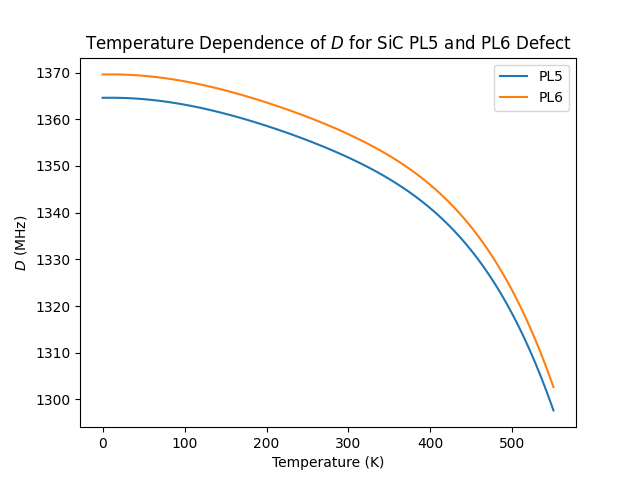
\includegraphics[width=0.49\textwidth]{figures/SiC-PL5PL6-D(T).png}
    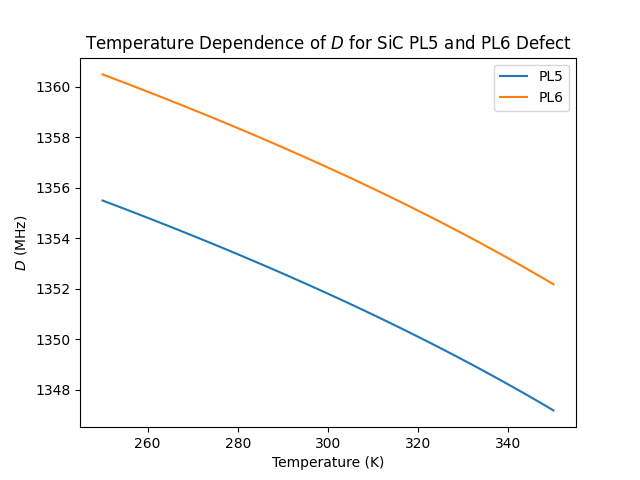
\includegraphics[width=0.49\textwidth]{figures/SiC-PL5PL6-D(T)-close.png}
    \caption{ZFS parameter $D$ temperature dependence for the PL5 and PL6 $S=1$ defect in SiC from 0-550 K (left) and 250-350 K (right). }\label{fig:PL5PL6DvsT}
\end{center}
\end{figure}

\td{Update the T dependence of PL5 and PL6 and regen the figure. Also update temp linear range in figure caption.}

In the simplest case thermometry is then achieved in the presence of a well known applied magnetic field. 

The measurement stems from the change of the value of
D mapped into the change of the oscillation frequency of the
relative variation of the photoluminescence intensity induced by the microwave pulse sequence.

Since the degeneracy is raised symmetrically, the value of $D$ is the average of the two resonant frequencies. The value of $D$ can then be mapped to a temperature. 

This is visualised in figure \ref{fig:pl6-3temps}. 

\begin{figure}[h]
    \begin{center}
        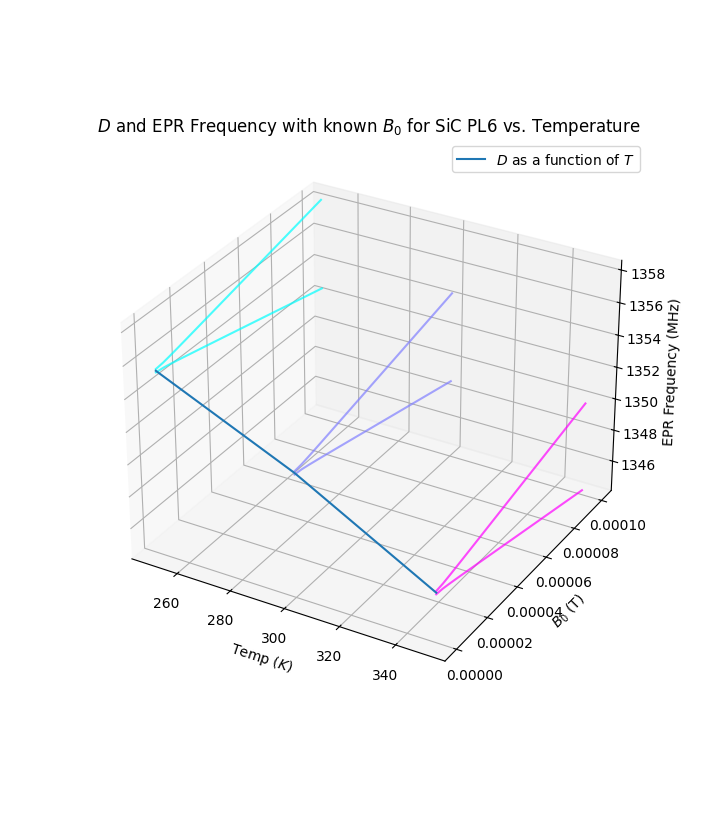
\includegraphics[width=0.8\textwidth]{figures/PL6-DvsT-3temps.png}
    \end{center}
    \caption{}\label{fig:pl6-3temps}
\end{figure}

In practice this \td{Write up the Ramsey Interference methods for c-axis and basal from Castello p18}. 

\section{$S= 3/2$ Thermometry}

\section{$S = 1$ Electometry}
\todo[inline]{Add matrix Hamiltonian as well as eigenval solutions. Include the formula for $\Delta \omega$ and dicuss the diminishing returns when $B\neq0$ or if $B \not\perp z$}

\section{$S=3/2$ Electrometry}




\section{Multimodality}
To develop our multimodal system we will start with a very simple model with the assumption that the applied $\vec{B}$ field is parallel to the defect axis. From there we will iterate our ensemble and work to reduce the number of assumptions.  


\subsection{$|\vec{B}|$ and $T$}
\cite{Degen2008}

\subsection{Angle Resolved $|\vec{B}|$ and $T$}
% We show that uniaxial color centers in silicon carbide with hexagonal lattice structure can be used to measure not only the strength but also the polar angle of the external magnetic field with respect to the defect axis with high precision. 
\cite{PhysRevApplied.4.014009}

\subsection{$\vec{B}$ and $T$}


\subsection{$|\vec{B}|$, $|\vec{E}|$ and $T$}
The influence of an $\vec{E}$ field parallel to the defect axis is indistinguishable from the influence of a change of temperature. Similarly, the influence of an $\vec{E}$ field perpendicular to the defect axis is indistinguishable from the influence of a $\vec{B}$ field parallel to the defect axis. The exception is when \td{When $B_0$ is smaller than ZFS E when the effects can be distinguished}... 

\begin{figure}[h]
    \begin{center}
        % \includegraphics[width=0.95\textwidth]{figures/}
        \missingfigure{2 plots. Both of a basline energy graph and showing the similarity of T and parallel E, and B and perp E.}
    \end{center}
    \caption{}\label{fig:}
\end{figure}


Thus, to extend the multi-modality to include the $\vec{E}$ field we must isolate the influence of the $\vec{E}$ field from the other environmental factors. 



\subsection{$\vec{B}$, $\vec{E}$ and $T$}
%
% This section should be written in standard scientific
% language. Standard techniques in your research field should not be
% written out in detail. In computational projects this section should
% be used to explain the algorithms used and the layout of the
% computational code. A copy of the actual code may be given in the
% appendices if appropriate.
%
% This section should emphasise the philosophy of the approach used and
% detail novel techniques. However please note: this section should not
% be a blow-by-blow account of what you did throughout the project. It
% should not contain large detailed sections about things you tried and
% found to be completely wrong! However, if you find that a technique
% that was expected to work failed, that is a valid result and should be
% included.
%
% Here logical structure is particularly important, and you may find
% that to maintain good structure you may have to present the
% explorations/calculations/computations/whatever in a different order
% from the one in which you carried them out.
%
%
% You might sometimes want to include multiple equations in one place
% \begin{eqnarray}
%   E &=& ma^{2} \\
%   E &=& mb^{2} \\
%   E &=& mc^{2}
% \end{eqnarray}
% You might want to include multiple equations in one place without
% numbering them
% \begin{eqnarray*}
%   E &=& ma^{2} \\
%   E &=& mb^{2} \\
%   E &=& mc^{2}
% \end{eqnarray*}
% You might want to include multiple equations in one place without
% numbering \emph{all} of them
% \begin{eqnarray}
%   E &=& ma^{2} \nonumber \\
%   E &=& mb^{2} \nonumber \\
%   E &=& mc^{2}
% \end{eqnarray}
%
% You might also want to include diagrams.  The example shows the use of
% the special command which allows existing pdf files to be included.
% You would normally keep your figures separate from the text.  These
% pictures might be images or pdf output from some program.
%
% Here, I created a figure which is centred and stretched to 30\% of the
% width of the page \verb+{0.30\hsize}+ and with the height stretched by
% the same amount \verb+{!}+ to preserve the aspect ratio. If you omit
% the extension (ie .eps, .ps or .pdf) on the file name then \LaTeX\ will
% pick up the postscript copy whereas pdflatex will automatically pick
% up the PDF version.
%
%
% \begin{figure}
%
% \begin{center}
%   \resizebox{0.30\hsize}{!}{
\includegraphics{crest.pdf}}
% \end{center}
%
% \caption{The coloured version of the University crest. The caption should explain exactly in some detail what is displayed in the table.}
% \label{fig:eucrest}
%
% \end{figure}
%
% You should find the file crest.pdf on this wiki.
%
% % note that labels do not need to include a description of the object
% % they are labelling but it can be helpful, eg \label{fig:figurename}.
%
% You can use a label on a figure to refer to it later. The university
% crest is in Figure~(\ref{fig:eucrest}). Note that you should not use
% phrases like ``the figure above'' or ``the following figure'' since
% \LaTeX\ may move the figure relative to the text if it cannot be fitted
% onto the current page. The figure on the next page is an example.
%
%
%
